\documentclass[UTF8,11pt,a4paper]{ctexart}

\usepackage[a4paper,left=1.45cm,right=1.45cm,top=1.55cm,bottom=1.65cm]{geometry}
\usepackage{amsmath,amssymb,bm}
\usepackage{graphicx}
\usepackage{booktabs,tabularx,array,multirow,longtable}
\usepackage{enumitem}
\usepackage[dvipsnames,svgnames]{xcolor}
\usepackage{tikz}
\usetikzlibrary{arrows.meta,positioning,calc,fit,shapes.geometric,shapes.misc,decorations.pathreplacing}
\usepackage[most]{tcolorbox}
\usepackage{hyperref}
\usepackage{caption}
\usepackage{subcaption}
\usepackage{float}
\usepackage{fancyhdr}
\usepackage{titlesec}
\usepackage{microtype}

\IfFontExistsTF{Times New Roman}{\setmainfont{Times New Roman}}{\setmainfont{Liberation Serif}}
\IfFontExistsTF{Noto Sans CJK SC}{\setCJKmainfont{Noto Sans CJK SC}}{}
\IfFontExistsTF{Noto Sans CJK SC}{\setCJKsansfont{Noto Sans CJK SC}}{}
\IfFontExistsTF{DejaVu Sans Mono}{\setmonofont{DejaVu Sans Mono}}{\setmonofont{Latin Modern Mono}}

\definecolor{DeepSkyBlue4}{HTML}{0B5CAD}
\hypersetup{colorlinks=true,linkcolor=DeepSkyBlue4,urlcolor=DarkOrange,citecolor=DeepSkyBlue4}
\graphicspath{{images/}}
\setlength{\parindent}{2em}
\setlength{\headheight}{14pt}
\setlength{\parskip}{0.22em}
\setlist[itemize]{leftmargin=2em,itemsep=0.2em,topsep=0.2em}
\setlist[enumerate]{leftmargin=2.2em,itemsep=0.2em,topsep=0.2em}
\renewcommand{\arraystretch}{1.2}
\captionsetup{font=small,labelfont=bf}

\definecolor{mainblue}{HTML}{0B5CAD}
\definecolor{softblue}{HTML}{EAF4FF}
\definecolor{darktext}{HTML}{1F2937}
\definecolor{softgray}{HTML}{F5F7FA}
\definecolor{accent}{HTML}{F59E0B}
\definecolor{goodgreen}{HTML}{2E7D32}
\definecolor{badred}{HTML}{B91C1C}
\definecolor{purple}{HTML}{6D5BD0}

\titleformat{\section}{\Large\bfseries\sffamily\color{mainblue}}{\thesection}{0.7em}{}
\titleformat{\subsection}{\large\bfseries\sffamily\color{darktext}}{\thesubsection}{0.6em}{}
\titleformat{\subsubsection}{\normalsize\bfseries\sffamily\color{darktext}}{\thesubsubsection}{0.55em}{}

\pagestyle{fancy}
\fancyhf{}
\fancyhead[L]{\small\sffamily Fractal Generative Models}
\fancyhead[R]{\small\sffamily \leftmark}
\fancyfoot[C]{\small\thepage}
\renewcommand{\headrulewidth}{0.4pt}

\newtcolorbox{infobox}[1]{enhanced,breakable,colback=softblue,colframe=mainblue!70!black,boxrule=0.8pt,arc=2mm,left=1.5mm,right=1.5mm,top=1mm,bottom=1mm,title=\bfseries #1}
\newtcolorbox{keybox}[1]{enhanced,breakable,colback=softgray,colframe=darktext!45,boxrule=0.6pt,arc=2mm,left=1.5mm,right=1.5mm,top=1mm,bottom=1mm,title=\bfseries #1}
\newtcolorbox{notebox}[1]{enhanced,breakable,colback=accent!8,colframe=accent!80!black,boxrule=0.7pt,arc=2mm,left=1.5mm,right=1.5mm,top=1mm,bottom=1mm,title=\bfseries #1}
\newcommand{\term}[1]{\textbf{\textcolor{mainblue}{#1}}}
\newcommand{\code}[1]{\texttt{#1}}
\newcommand{\x}{\bm{x}}

\begin{document}

\section{论文基本信息}

\begin{center}
\begin{tabularx}{0.92\linewidth}{>{\bfseries}p{0.18\linewidth}X}
\toprule
题目 & \textit{Fractal Generative Models}（分形生成模型）\\
作者 & Tianhong Li, Qinyi Sun, Lijie Fan, Kaiming He\\
关键词 & Fractal, Generative Model, Autoregressive Model, Pixel-by-pixel Generation\\
一句话概括 & 把一个完整的生成模型抽象为“原子生成模块”，再递归调用它，形成具有自相似结构的分形生成架构。\\
\bottomrule
\end{tabularx}
\end{center}

\begin{infobox}{摘要要点}
传统模块化通常把神经网络分解为层、残差块或 Transformer block。本文进一步提出：不仅网络层可以模块化，\term{生成模型本身}也可以被当成模块。递归地调用这些原子生成模块，就会形成类似数学分形的自相似结构。作者以自回归模型作为原子模块，在逐像素图像生成任务上验证了似然估计和生成质量。
\end{infobox}

\section{核心直觉：为什么叫“分形生成模型”}\label{sec:core}

\subsection{从普通模块化到生成模型模块化}

\begin{figure}[H]
\centering
\begin{tikzpicture}[node distance=1.1cm,>=Latex]
\tikzstyle{blk}=[draw,rounded corners,align=center,minimum width=2.6cm,minimum height=0.9cm,fill=softblue]
\tikzstyle{big}=[draw,rounded corners,align=center,minimum width=3.4cm,minimum height=1.1cm,fill=accent!12]
\node[blk] (layer) {神经网络层\\Layer};
\node[blk,right=of layer] (block) {残差/Transformer\\Block};
\node[big,right=of block] (model) {生成模型\\Generative Model};
\draw[->,thick,mainblue] (layer) -- node[above,font=\small]{组合} (block);
\draw[->,thick,mainblue] (block) -- node[above,font=\small]{进一步抽象} (model);
\node[below=0.45cm of model,align=center,text width=4.0cm] {本文的关键提升：把\textbf{整个生成模型}当作可以递归调用的模块。};
\end{tikzpicture}
\caption{模块化层次的提升：从 layer/block 到 generative model。}
\end{figure}

DNN 中的 layer、ResNet 中的 residual block、Transformer 中的 attention block 都是模块化的例子。本文的创新点是把“一个生成步骤”甚至“一个生成模型”整体作为模块。这样，父生成器可以调用多个子生成器，子生成器继续调用更小的生成器，形成递归结构。

\subsection{分形的类比}

\begin{figure}[H]
\centering
\begin{tikzpicture}[scale=0.95]
\newcommand{\tri}[4]{\fill[#4] (#1,#2+1.6*#3) -- (#1-1.4*#3,#2-0.8*#3) -- (#1+1.4*#3,#2-0.8*#3) -- cycle;}
\newcommand{\hole}[3]{\fill[white] (#1,#2+0.45*#3) -- (#1-0.45*#3,#2-0.32*#3) -- (#1+0.45*#3,#2-0.32*#3) -- cycle;}
\tri{-4}{0}{1}{mainblue!60} \hole{-4}{0}{1}
\tri{0}{0}{1}{mainblue!60} \hole{0}{0}{1}
\foreach \x/\y in {-0.7/-0.4,0.7/-0.4,0/0.8}{\hole{\x}{\y}{0.5}}
\tri{4}{0}{1}{mainblue!60} \hole{4}{0}{1}
\foreach \x/\y in {3.3/-0.4,4.7/-0.4,4/0.8}{\hole{\x}{\y}{0.5}}
\foreach \x/\y in {3.65/-0.6,4.35/-0.6,4/-0.0,4.35/0.6,3.65/0.6,4/1.2}{\hole{\x}{\y}{0.22}}
\node at (-4,-1.7){第 1 层};
\node at (0,-1.7){第 2 层};
\node at (4,-1.7){第 3 层};
\end{tikzpicture}
\caption{数学分形的核心特征是递归规则与跨尺度自相似。分形生成模型将这一思想迁移到生成模型结构。}
\end{figure}

分形并不是简单的“很多层”，而是\term{同一种生成规则在不同尺度上重复出现}。在本文中，不同层级的生成器具有相似的功能：接收上一级输出，产生若干下一级输入，直到最终生成像素。

\subsection{递归的最简单例子：阶乘}

\begin{notebox}{递归三要素}
递归通常包含三部分：问题定义、基本情况、递归调用。阶乘满足
\begin{equation}
0!=1,\qquad n!=n\times(n-1)!,\quad n>0.
\end{equation}
分形生成模型中的递归不是计算一个数，而是递归地生成数据块。
\end{notebox}

\section{背景模型：自回归与扩散}

\subsection{自回归模型}

自回归模型的基本思想是按照某个顺序逐步生成数据。对于序列 $x_1,x_2,\ldots,x_N$，联合分布可以写成
\begin{equation}
    p(x_1,x_2,\ldots,x_N)=\prod_{i=1}^{N}p(x_i\mid x_1,x_2,\ldots,x_{i-1}).
\end{equation}
在图像中，如果直接把所有像素排成一个长序列，那么序列会非常长，计算代价非常高。

\begin{figure}[H]
\centering
\begin{tikzpicture}[>=Latex]
\foreach \i/\v in {0/128,1/130,2/132,3/?}{
    \pgfmathsetmacro{\xx}{mod(\i,2)*1.2}
    \pgfmathsetmacro{\yy}{-floor(\i/2)*1.0}
    \draw[fill=softgray] (\xx,\yy) rectangle +(1.2,1.0);
    \node at (\xx+0.6,\yy+0.5){\v};
}
\draw[->,thick,mainblue] (1.55,-0.5) -- (3.1,-0.5) node[midway,above]{条件生成};
\node[draw,rounded corners,fill=softblue,align=left,text width=6cm] at (6.3,-0.5){
$p(x_{1,1}=128)$ 先给第一个像素；\\
$p(x_{1,2}\mid x_{1,1})$ 再给第二个像素；\\
$p(x_{2,1}\mid x_{1,1},x_{1,2})$ 继续；\\
最后预测 $p(x_{2,2}\mid \text{前三个像素})$。};
\end{tikzpicture}
\caption{逐像素自回归生成的直观示例。}
\end{figure}

\subsection{扩散模型}

扩散模型通常包含“逐步加噪”和“逐步去噪”两个方向。加噪过程把清晰图像变成噪声，去噪过程从噪声逐步恢复图像。它的模块化单元更接近“生成步骤”：每一步由一个神经网络预测噪声或去噪方向。

\begin{center}
\begin{tabularx}{0.86\linewidth}{cXc}
\toprule
阶段 & 作用 & 模块含义\\
\midrule
加噪 & 逐步向图像添加高斯噪声，最终得到接近纯噪声的样本 & 前向过程\\
去噪 & 从噪声出发，逐步预测并去除噪声，恢复清晰图像 & 生成过程\\
\bottomrule
\end{tabularx}
\end{center}

\section{相关工作整理}

\begin{longtable}{p{0.18\linewidth}p{0.76\linewidth}}
\toprule
\textbf{方向} & \textbf{核心内容与本文关系}\\
\midrule
分形 & 自然界中云、树枝、雪花、晶体、染色质和蛋白质等都可能呈现分形或近分形特征。本文借用“递归规则 + 自相似结构”的思想来设计生成模型。\\
层次化表征 & 传统视觉中的可转向滤波器、拉普拉斯金字塔、SIFT，以及深度学习中的 SPPNet、FPN、Swin Transformer 都强调多尺度表示；但它们通常不是严格的递归生成结构。\\
层次化生成模型 & VQ-VAE、latent codes、MegaByte、级联扩散、尺度空间自回归等方法也有层次性；本文不同点在于将生成模型本身当作可递归调用的原子模块。\\
模块化神经架构 & GoogleNet 的 Inception module、ResNet 的 residual block、Transformer block、MAR、FractalNet 都体现模块化思想；本文把模块化层次提升到“完整生成模型”级别。\\
\bottomrule
\end{longtable}

\section{分形生成模型的数学形式}\label{sec:math}

\subsection{分形生成器}

设第 $i$ 层生成器为 $g_i$，上一层给出一个输出 $x_i$。分形生成器的作用是为下一层产生一组数据：
\begin{equation}
    \{x_{i+1}\}=g_i(x_i).
\end{equation}
这里的关键是：一个输入可以产生多个输出，因此随着层级加深，输出数量可以指数增长。

\begin{figure}[H]
\centering
\begin{tikzpicture}[>=Latex,node distance=0.9cm]
\tikzstyle{gen}=[draw,rounded corners,fill=softblue,minimum width=1.3cm,minimum height=0.8cm,align=center]
\tikzstyle{outnode}=[circle,draw,fill=accent!20,minimum size=0.55cm]
\node[outnode] (x0) {$x_i$};
\node[gen,right=1.1cm of x0] (g) {$g_i$};
\draw[->,thick] (x0)--(g);
\foreach \j/\dy in {1/0.9,2/0.3,3/-0.3,4/-0.9}{
    \node[outnode,right=2.0cm of g,yshift=\dy cm] (y\j) {$x_{i+1}^{(\j)}$};
    \draw[->,thick,mainblue] (g.east) -- (y\j.west);
}
\node[draw,dashed,rounded corners,fit=(y1)(y4),label=right:{\small 下一层输入集合}] {};
\end{tikzpicture}
\caption{一个分形生成器将一个上级输出展开为多个下级输出。}
\end{figure}

如果每层都产生 $k$ 个输出，递归 $n$ 层后可以覆盖 $k^n$ 个基本变量。也就是说，模型只需要 $n=\log_k N$ 层，就能组织 $N$ 个变量。

\subsection{把自回归模型作为分形生成器}

目标是建模 $N$ 个随机变量的联合分布。若 $N=k^n$，直接用一个超长自回归模型会很贵。分形思想将其分为 $k$ 个子块：
\begin{equation}
\begin{aligned}
 p(x_1,\ldots,x_{k^n})
 &=\prod_{i=1}^{k}p\Big(
 x_{(i-1)k^{n-1}+1},\ldots,x_{ik^{n-1}}
 \mid x_1,\ldots,x_{(i-1)k^{n-1}}
 \Big).
\end{aligned}
\end{equation}
每个条件分布仍然包含 $k^{n-1}$ 个变量，于是继续交给下一层自回归模型处理。反复递归后，每一层只面对长度大约为 $k$ 的可控序列。

\begin{infobox}{公式含义}
上式不是简单地把一串像素切开，而是把“建模一个巨大联合分布”的任务分解成多个条件子问题。父模型负责粗粒度依赖，子模型负责更细粒度依赖；同一层的多个子问题可以并行处理，这是效率提升的重要来源。
\end{infobox}

\subsection{复杂度直觉}

单个长序列 Transformer 的注意力计算通常接近 $O(N^2)$。如果把 $N=k^n$ 个变量递归分解，模型在每层只处理较短序列，并把大量细粒度子问题拆到多个小模型中。于是它获得了两个好处：
\begin{itemize}
    \item \term{计算更可控}：避免单个模型直接处理全部像素序列。
    \item \term{结构更贴近图像}：图像本身具有局部块、子图像、全局布局等多尺度结构。
\end{itemize}

\section{图像生成实例}

\subsection{逐像素生成的挑战}

RGB 图像的每个像素有 3 个通道，$256\times256$ 图像共有 $196608$ 个通道值。如果按普通自回归方式从第一个值一直排到最后一个值，序列过长，训练和采样都很困难。更重要的是，图像不是天然的一维文本序列，直接线性展开会破坏二维结构。

\subsection{架构：父生成器到子生成器}

\begin{figure}[H]
\centering
\begin{tikzpicture}[>=Latex,node distance=0.8cm]
\tikzstyle{token}=[circle,draw,fill=purple!25,minimum size=0.62cm]
\tikzstyle{block}=[draw,rounded corners,fill=softblue,minimum width=6.5cm,minimum height=0.85cm,align=center]
\node[token] (prev) {上};
\node[block,below=of prev] (g1) {$g_1$: Transformer 处理粗粒度图像块};
\node[block,below=of g1] (g2) {$g_2$: Transformer 处理子块};
\node[block,below=of g2] (g3) {$g_3/g_4$: 逐步细化到像素与 RGB 通道};
\draw[->,thick] (prev) -- (g1);
\draw[->,thick] (g1) -- (g2);
\draw[->,thick] (g2) -- (g3);
\foreach \i in {-2,-1,0,1,2}{
    \node[token,below=0.9cm of g3,xshift=\i*1.3cm] (o\i) {};
    \draw[->,thick,mainblue] (g3.south) -- (o\i.north);
}
\node[below=1.8cm of g3,align=center] {输出给下一层生成器，最终得到像素值};
\end{tikzpicture}
\caption{分形图像生成架构的简化重绘：每一层生成多个下一层输入。}
\end{figure}

在每个分形层级中，自回归模型接收上一层生成器的输出，并结合对应图像块或子块，经过 Transformer blocks 后产生下一层生成器所需的一组输出。最后一层用很轻量的 Transformer 对 RGB 通道做自回归预测，并使用 256 类交叉熵损失。

\subsection{AR 与 MAR 两种实例}

\begin{center}
\begin{tabularx}{0.92\linewidth}{p{0.18\linewidth}p{0.34\linewidth}X}
\toprule
模型 & 生成顺序 & 特点\\
\midrule
FractalAR & raster order，类似 GPT 的因果 Transformer & 顺序明确、实现直观，但生成顺序固定。\\
FractalMAR & random order，类似 BERT 的双向 Transformer + masked autoregressive 思想 & 随机顺序更灵活，实验中生成质量更好。\\
\bottomrule
\end{tabularx}
\end{center}

\subsection{训练与生成策略}

\begin{keybox}{训练：广度优先}
训练时从顶层自回归模型开始，逐层向下传递到像素级表示。最后一层预测 RGB 值，采用交叉熵损失；损失通过所有层级反向传播，实现端到端训练。
\end{keybox}

\begin{keybox}{生成：深度优先}
生成时从顶层开始，沿着某个分支不断向下，直到真实像素值被采样出来，再回到其他分支。这种深度优先遍历适合递归架构。
\end{keybox}

\section{实验整理}\label{sec:exp}

实验主要在 ImageNet $64\times64$ 与 $256\times256$ 上进行，评价维度包括似然估计、生成质量和条件逐像素预测。

\subsection{模型配置与计算量}

\begin{table}[H]
\centering
\small
\caption{不同分辨率下大模型的层级配置与计算量。}
\begin{tabular}{llcc}
\toprule
类别 & 层级 & $64\times64\times3$ & $256\times256\times3$\\
\midrule
\multirow{4}{*}{Seq. len.} & $g_1$ & 256 & 256\\
 & $g_2$ & 16 & 16\\
 & $g_3$ & 3 & 16\\
 & $g_4$ & -- & 3\\
\midrule
\multirow{4}{*}{\#layers} & $g_1$ & 32 & 32\\
 & $g_2$ & 8 & 8\\
 & $g_3$ & 3 & 4\\
 & $g_4$ & -- & 1\\
\midrule
\multirow{4}{*}{hidden dim} & $g_1$ & 1024 & 1024\\
 & $g_2$ & 512 & 512\\
 & $g_3$ & 128 & 256\\
 & $g_4$ & -- & 64\\
\midrule
\multirow{4}{*}{\#params (M)} & $g_1$ & 403 & 403\\
 & $g_2$ & 25 & 25\\
 & $g_3$ & 0.6 & 3\\
 & $g_4$ & -- & 0.1\\
\midrule
\multirow{4}{*}{\#GFLOPs} & $g_1$ & 215 & 215\\
 & $g_2$ & 208 & 208\\
 & $g_3$ & 15 & 419\\
 & $g_4$ & -- & 22\\
\bottomrule
\end{tabular}
\end{table}

从表中可以看到，$256\times256$ 相比 $64\times64$ 增加了更深的细粒度层级，但并不是把所有像素直接放到同一个巨大序列里。因此论文强调：得益于分形设计，$256\times256$ 的总计算量约为 $64\times64$ 的两倍。

\subsection{似然估计}

\begin{table}[H]
\centering
\small
\caption{ImageNet $64\times64$ 无条件生成上的似然估计与计算量比较。NLL 单位为 bits/dim，越低越好。}
\begin{tabular}{lccccl}
\toprule
模型 & $g_1$ & $g_2$ & $g_3$ & \#GFLOPs & NLL $\downarrow$\\
\midrule
AR, full-length & 12288 & -- & -- & 29845 & N/A\\
MAR, full-length & 12288 & -- & -- & 29845 & N/A\\
AR, 2-level & 4096 & 3 & -- & 5516 & 3.34\\
MAR, 2-level & 4096 & 3 & -- & 5516 & 3.36\\
FractalAR (3-level) & 256 & 16 & 3 & 438 & 3.14\\
FractalMAR (3-level) & 256 & 16 & 3 & 438 & 3.15\\
\bottomrule
\end{tabular}
\end{table}

\begin{notebox}{读表结论}
更多分形层级带来了更低的计算量和更好的似然估计。尤其是 3-level 模型把 GFLOPs 从数千量级降到 438，同时 NLL 也更好。
\end{notebox}

\subsection{生成质量}

\begin{table}[H]
\centering
\small
\caption{ImageNet $64\times64$ 条件生成质量对比。FID 越低越好。}
\begin{tabular}{llc}
\toprule
模型 & 类型 & FID $\downarrow$\\
\midrule
iDDPM & diffusion & 2.92\\
StyleGAN-XL & GAN & \textbf{1.51}\\
Consistency Model & consistency & 4.70\\
MAR & AR+diffusion & 2.93\\
\midrule
FractalAR & fractal & 5.30\\
FractalMAR & fractal & 2.72\\
\bottomrule
\end{tabular}
\end{table}

\begin{table}[H]
\centering
\small
\caption{ImageNet $256\times256$ 生成质量对比。}
\begin{tabular}{lccccc}
\toprule
模型 & 类型 & 参数量 & FID $\downarrow$ & IS $\uparrow$ & Precision $\uparrow$\\
\midrule
BigGAN-deep & GAN & 160M & 6.95 & 198.2 & \textbf{0.87}\\
GigaGAN & GAN & 569M & 3.45 & 225.5 & 0.84\\
StyleGAN-XL & GAN & 166M & 2.30 & 265.1 & 0.78\\
ADM & diffusion & 554M & 4.59 & 186.7 & 0.82\\
Simple diffusion & diffusion & 2B & 3.54 & 205.3 & --\\
VDM++ & diffusion & 2B & 2.12 & 267.7 & --\\
SiD$^2$ & diffusion & -- & \textbf{1.38} & -- & --\\
JetFormer & AR+flow & 2.8B & 6.64 & -- & 0.69\\
\midrule
FractalMAR-B & fractal & 186M & 11.80 & 274.3 & 0.78\\
FractalMAR-L & fractal & 438M & 7.30 & 334.9 & 0.79\\
FractalMAR-H & fractal & 848M & 6.15 & \textbf{348.9} & 0.81\\
\bottomrule
\end{tabular}
\end{table}

\begin{infobox}{生成质量的理性解读}
FractalMAR 在 $64\times64$ 上接近强基线，并在逐像素框架中取得较好结果；在 $256\times256$ 上，FID 仍落后于顶级 GAN/扩散模型，但它展示了逐像素生成路线的可行性。换言之，本文更像是提出一种新范式，而不是单纯刷新所有指标。
\end{infobox}

\subsection{定性结果}

\begin{figure}[H]
\centering
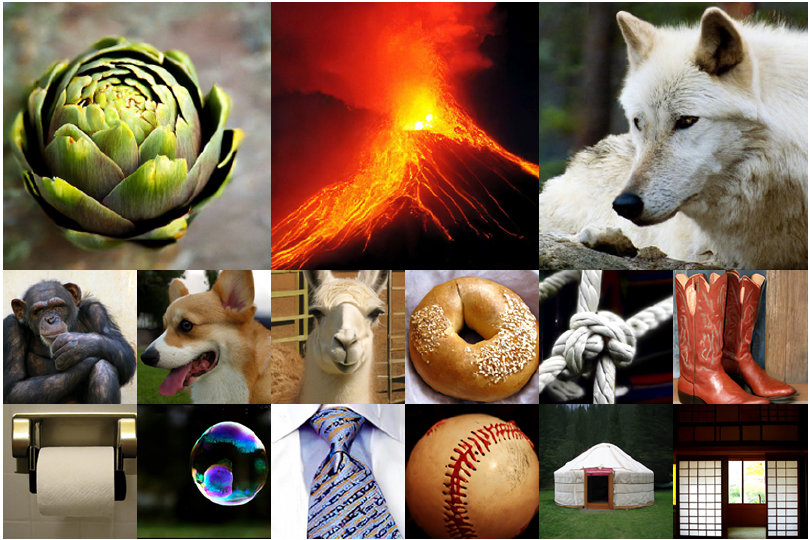
\includegraphics[width=0.85\linewidth]{generated_samples.png}
\caption{课件中保留的 ImageNet $256\times256$ 逐像素生成结果。}
\end{figure}

\begin{figure}[H]
\centering
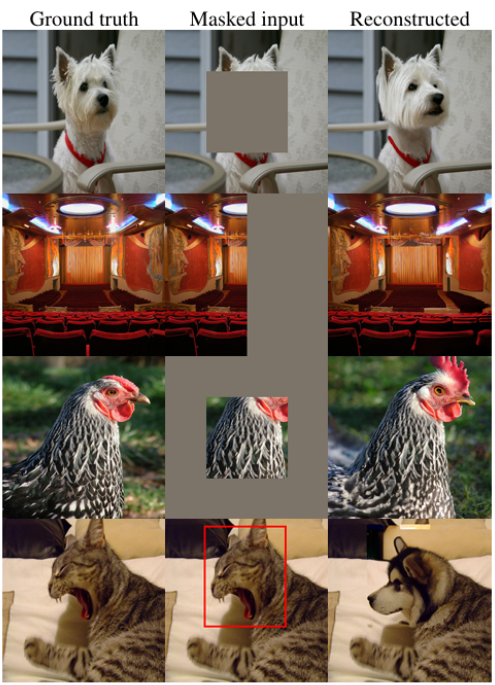
\includegraphics[width=0.62\linewidth]{conditional_prediction.png}
\caption{条件逐像素预测示例：包含图像修复、外推、反裁剪和类别条件编辑等任务。}
\end{figure}

\section{个人点评与创新点}

\subsection{论文创新点}

\begin{enumerate}
    \item \term{模块化层次提升}：不是把网络层当模块，而是把完整生成模型当作原子模块。
    \item \term{递归生成架构}：通过父生成器调用子生成器，形成多尺度、自相似结构。
    \item \term{逐像素生成的新可能}：在不依赖 tokenizer 的情况下，直接对原始像素进行生成建模。
    \item \term{效率与结构兼顾}：把长序列建模拆成分治式的层级子问题，降低单层序列长度。
\end{enumerate}

\subsection{值得继续思考的方向}

\begin{notebox}{可作为自己汇报中的创新观点}
分形生成模型的潜力不只在图像。只要数据存在“整体由局部组成、局部又有类似结构”的特征，就可以考虑分形生成。比如点云、蛋白质结构、图神经网络中的大图生成、机器人多层动作规划，都可能尝试把“子结构生成器”递归嵌入到“整体生成器”中。
\end{notebox}

\subsection{局限性}

\begin{itemize}
    \item 目前主要以图像逐像素生成作为验证场景，其他非顺序结构数据上的效果仍需要进一步实验。
    \item 生成质量并未全面超过顶级扩散模型或 GAN，尤其在 $256\times256$ FID 上仍有差距。
    \item 递归层级、子块划分、AR/MAR 选择等设计空间较大，工程调参成本不低。
\end{itemize}

\end{document}
